% AnchorMTM full draft: Sections 1-4 = collaborator version of 2026-11-02 (unchanged);
% Sections 5-7 drafted 2026-11-03 from the evaluation of the 2026-10-30 version (commit 91e1fb8).
% Overleaf: upload this folder, main file main.tex, compiler pdfLaTeX.
% Build: tectonic -X compile --keep-logs method_anchor_figures_updated_en.tex
% Unchanged companion: method_anchor_single_parameter_supplement.tex/.pdf.
% Changes: ANCHORMTM_SINGLE_PARAMETER_VALIDATION.md.
\documentclass[review]{vgtc}
\usepackage[T1]{fontenc}
\usepackage{mathptmx}
\usepackage{booktabs}
\usepackage{cite}
\usepackage{amsmath,amssymb,amsthm}
\usepackage{flafter}
\usepackage[ruled,vlined]{algorithm2e}
\SetKwInput{KwData}{Data}
\SetKwInput{KwResult}{Result}
\SetKwProg{Fn}{Function}{:}{}
\SetKw{KwReturn}{return}
\SetKw{KwBreak}{break}
\SetKwFunction{Construct}{ConstructTemporalMap}
\SetKwFunction{Refine}{RefineOrder}
\SetKwFunction{Barriers}{OptimalBarriers}
\SetAlFnt{\small}
\SetAlCapFnt{\small\bfseries}
\SetAlCapNameFnt{\small\bfseries}
\SetAlCapSkip{3pt}
\DontPrintSemicolon
\setcounter{secnumdepth}{3}
\newtheorem{theorem}{Theorem}
\newtheorem{lemma}{Lemma}
\newtheorem{proposition}{Proposition}
\newcommand{\dtop}{d_{\mathrm{top}}}
\newcommand{\lca}{\operatorname{lca}}
\newcommand{\nroe}{\mathrm{NROE}}
\newcommand{\pos}[1]{\left[#1\right]^+}
\title{AnchorMTM: Spatially Anchored Merge Tree Maps\\for Time-Varying Scalar Fields}
\author{Anonymous Authors}
\onlineid{0}
\vgtccategory{Research}
\vgtcinsertpkg
\hypersetup{pdftitle={AnchorMTM: Spatially Anchored Merge Tree Maps for Time-Varying Scalar Fields},pdfauthor={Anonymous Authors}}
\abstract{Temporal merge tree maps summarize evolving scalar topology, but their display coordinates need not correspond to a common spatial direction. AnchorMTM links these coordinates to a fixed reference estimated once from matched extremum motion across a 2D or 3D sequence. The leading eigenvector of the motion scatter matrix maximizes squared projected motion; a physically meaningful direction can alternatively be supplied. This standard estimation step provides targets for topology-budgeted layout rather than a separate direction-optimization contribution. A finite heuristic search seeks a leaf order with small worst reference displacement under a declared merge-level error budget. Exact fixed-order displacement and optimal-barrier evaluations support this search, followed by a capped quadratic program that balances spatial anchoring and projected motion with relative geometry and interval centering. Scalar-profile reconstruction produces the temporal map. Three certified bounds explain unavoidable position error under exact topology, finite widths, and bounded topological error; they benchmark layouts rather than prune the search. Continuous feasibility and actual rendered errors are reported separately.}
\keywords{Time-varying scalar fields, merge tree maps, spatial anchoring, topology preservation, constrained layout.}
\teaser{
\centering
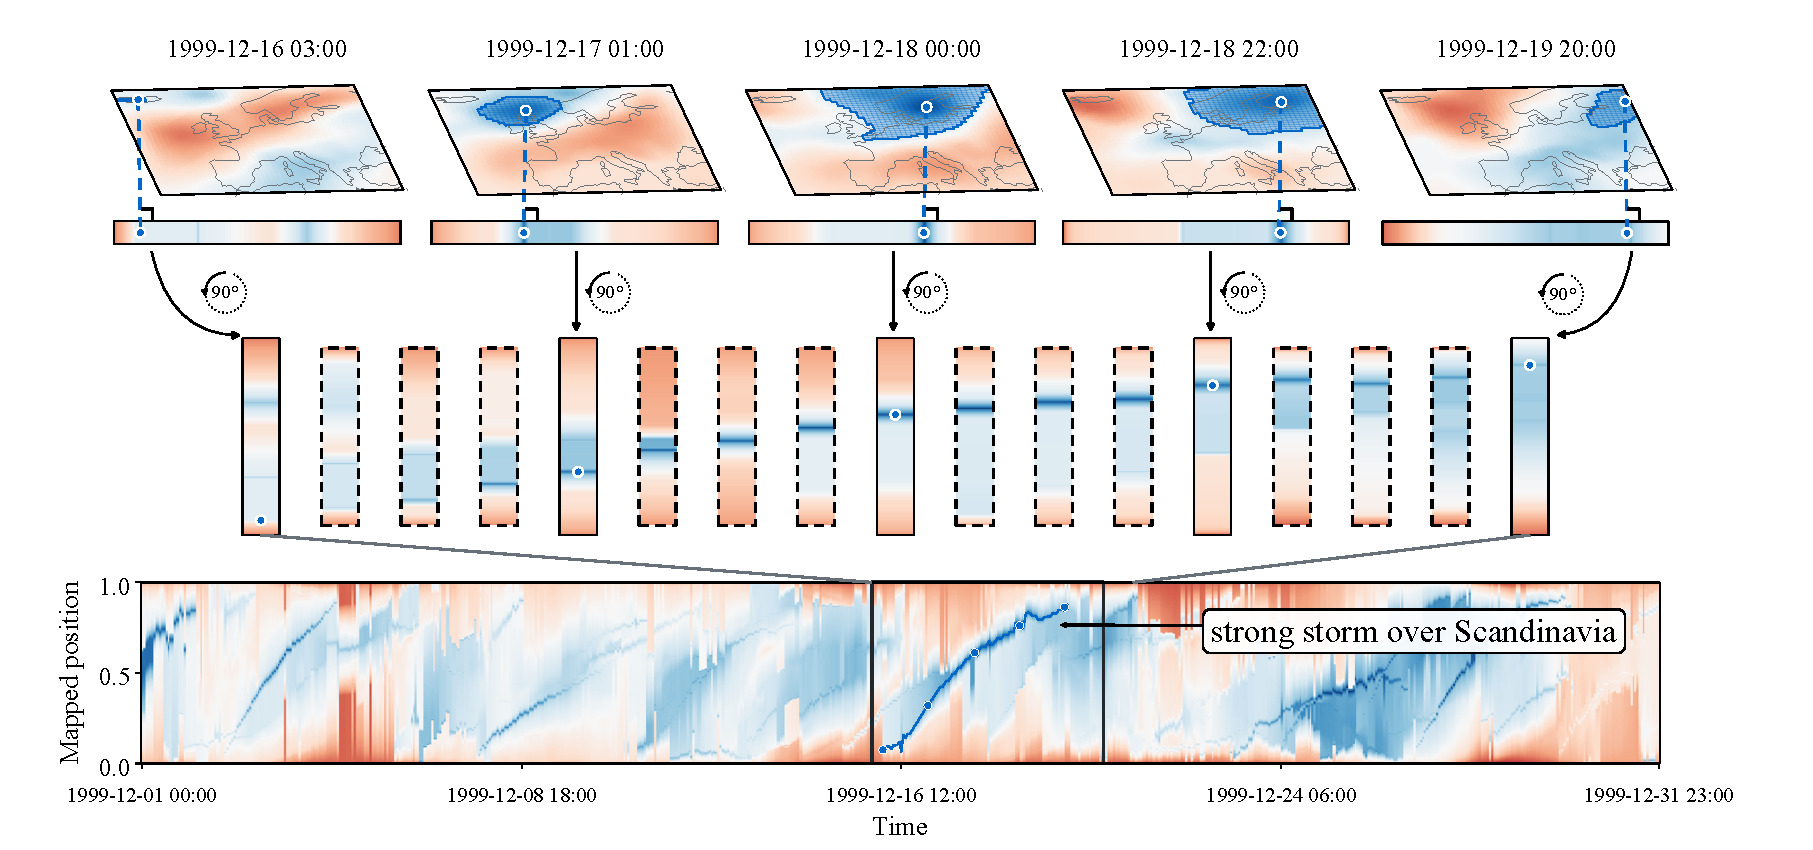
\includegraphics[width=\linewidth]{figures/anchor_storms_overview.pdf}
\par
\refstepcounter{figure}\label{fig:storms_overview}
{\captionfonts\raggedright\noindent\figurename~\thefigure: Storms example linking spatial feature supports to a temporal map ($\varepsilon=5\%$). Top: five snapshots of one matched extremum and their scalar profiles; blue outlines mark its leaf-arc supports, and dashed guides link the extrema to their displayed profile anchors. Middle: the profiles rotated by $90^\circ$; dashed borders distinguish sampled intermediate frames. Bottom: the full 744-frame map, with the selected storm-related region outlined and the matched feature's displayed positions marked in blue.\par}

}
\begin{document}
\firstsection{Introduction}
\maketitle
\raggedbottom
\setlength{\emergencystretch}{1.5em}
2D and 3D time-varying scalar fields describe evolving phenomena such as pressure systems, combustion structures, and flow features. Their analysis requires understanding where features occur, how they move along a relevant spatial direction, and how their hierarchical relationships change throughout a sequence. Extrema and component merges describe this evolving scalar structure, while spatial coordinates connect it to the physical domain. A temporal overview should bring these aspects together. Figure~\ref{fig:storms_overview} illustrates how spatial supports and reference positions connect to scalar profiles and the resulting temporal map.

Animation preserves the spatial view at each instant, but comparison between distant times requires navigation and memory. Small multiples expose observations simultaneously at the cost of screen space. Static temporal summaries allocate one display axis to time and compress the spatial domain into the remaining axis~\cite{Tversky:2002:Animation,Robertson:2008:Animation,Bach:2017:STC}. Spatial linearization makes long sequences accessible in one image; the meaning of its 1D coordinate determines which spatial questions the overview can support.

Merge tree maps organize this compression around scalar features and their hierarchy. Temporal Merge Tree Maps (TMTM) linearize augmented merge trees into scalar profiles aligned across time~\cite{Koepp:2023:TMTM}. Minima and intervening barriers encode extrema and merge levels, exposing scalar structure and its temporal evolution. Spatiotemporal Merge Tree Maps (ST-MTM) incorporate relative spatial distances and temporal position constraints into a geometry-aware layout~\cite{STMTM:2026}. These methods provide the foundation for compact overviews of temporal scalar topology.

A display coordinate chosen for hierarchy, relative distance, or temporal alignment need not correspond to a fixed physical direction. Its position cannot then be read directly as longitude or distance along a flow axis, and its changes need not represent motion along that direction. Relative geometry supplies spatial relationships but leaves the absolute coordinate origin undetermined. The remaining question is how to give the temporal map a consistent spatial reference while retaining its hierarchical information.

We introduce \emph{Automatic Spatial Anchoring}: estimating one dominant motion direction from matched extrema over the full sequence, assigning projected targets in that shared coordinate system, and placing display anchors nearby as constraints permit. A task-specific physical direction remains an option. The direction estimator is a standard leading-eigenvector calculation; our contribution is its connection to merge-tree layout, explicit topology budgets and position bounds. A reference order can conflict with topology when the projected leaves of different subtrees interleave while exact topology requires contiguous subtree blocks. Finite feature widths introduce further packing constraints. Allowing bounded topological error releases some ordering restrictions and exposes a controlled position--topology trade-off.

AnchorMTM, \emph{Spatially Anchored Merge Tree Maps}, follows one construction: extract and match features, construct a fixed reference, seek a topology-admissible leaf order, optimize anchors within legal intervals, and reconstruct scalar profiles on a shared temporal axis. Exact Mode and Budgeted Mode use the same layout framework with different admissible merge errors. Position bounds then explain the discrepancy that topology and finite widths make unavoidable.

Our main contributions are as follows:
\begin{itemize}
\setlength{\itemsep}{2pt}
\setlength{\parsep}{0pt}
\item We formulate automatic spatial anchoring for temporal merge tree maps, using a single direction estimated from matched extremum motion to establish consistent spatial references across a 2D or 3D sequence.
\item We develop a topology-budgeted layout framework that combines reference-aware leaf ordering with capped spatiotemporal anchor optimization. Exact and budgeted modes share the same framework, with explicit position and merge-level error accounting.
\item We establish certified position bounds that quantify unavoidable reference displacement under exact topology, finite feature widths, and bounded topological error.
\end{itemize}

\section{Related Work}\label{sec:related}
\subsection{Spatially Referenced Temporal Visualization}
Static temporal displays expose distant observations simultaneously, while animation retains the spatial view of each instant; their usefulness depends on the analytical task~\cite{Tversky:2002:Animation,Robertson:2008:Animation}. Generalized space--time cubes describe the transformations connecting such views~\cite{Bach:2017:STC}. In compressed temporal overviews, the spatial coordinate determines which location and motion relationships remain directly interpretable.

Hovm\"oller diagrams retain a selected physical coordinate and summarize the other dimensions~\cite{Hovmoller:1949}. Geographic orderings and space-filling curves instead traverse the domain~\cite{Guo:2006:SpatialOrder,Dafner:2000:CSFC}. Dynamic Volume Lines and data-driven curves extend spatial traversal to volumetric comparison and scalar-aware ordering~\cite{Weissenboeck:2019:DVL,Zhou:2021:DSF}. A traversal can retain spatial neighborhoods, but its 1D coordinate is generally different from a fixed projection, and traversal adjacency alone does not enforce the merge hierarchy.

1D projections organize spatiotemporal phenomena~\cite{Franke:2021:1DP}, and MotionRugs expose collective behavior of moving entities~\cite{Buchmueller:2019:MR}. More generally, an embedding trades original-domain relationships against its display organization~\cite{Nonato:2019:MP}. Relative proximity does not determine an absolute coordinate. AnchorMTM assigns fixed projection targets to topological features and quantifies their displacement under hierarchical and interval constraints, combining spatial reference with a temporal topology overview.

\subsection{Topology-Based Temporal Maps and Geometry-Aware Layouts}
Topology-based visualization organizes scalar structures through connectivity~\cite{Heine:2016:Survey}. Landscapes and landscape profiles express hierarchies through terrain or 1D scalar representations~\cite{Weber:2007:TL,Oesterling:2013:TLP}, with geometry-preserving and temporally coherent extensions~\cite{Beketayev:2012:GPTL,Herick:2020:TCTL}. These representations connect scalar values and feature relationships in a compact view.

TMTM emphasizes intact topological features and temporal alignment in static merge-tree maps~\cite{Koepp:2023:TMTM}. ST-MTM incorporates relative spatial geometry and temporal position constraints~\cite{STMTM:2026}. These priorities give spatial relationships and coherence a role in the map, while leaving its display coordinate free to differ from a fixed physical direction. AnchorMTM estimates a shared direction from extremum motion, or accepts a physical direction, and couples that reference to topology-budgeted layout and certified position bounds. It reuses the established profile and scalar-filling foundation.

Hierarchy-constrained leaf ordering traditionally minimizes adjacent dissimilarity~\cite{BarJoseph:2001:OLO}; target-order reordering studies related tree-consistent permutations~\cite{Bulteau:2022:RT}. Separation-constrained layouts control geometric overlap and displacement~\cite{Dwyer:2006:IPSEP,Li:2019:SOI}. AnchorMTM couples these layout concerns to fixed spatial targets. Its exact-topology point-order bound has a closed form, whereas finite-width candidate ordering remains heuristic.

Merge-tree comparison depends on the descriptors and correspondences used~\cite{Yan:2021:Survey}. Labelled cophenetic/interleaving comparisons support fixed-identity merge-level accounting~\cite{Munch:2019:LINF,Gasparovic:2024:IID}, and ordered merge trees connect scalar curves to monotone interleaving distances~\cite{Beurskens:2025:OMT}. We use fixed labels to measure displayed merge error. The optimal-barrier subproblem relates to minimax ultrametric fitting~\cite{Farach:1995:RM}, with the additional restriction that one linear order induces every displayed merge.

\section{Background}\label{sec:background}
\subsection{Augmented Merge Trees and Feature Supports}
For a sampled 2D or 3D field $f_t:D\to\mathbb{R}$, the merge tree $T_t$ records sublevel-set connectivity: minima create components and saddles join them as the threshold increases. Negating the field gives the split-tree convention. Critical points are supernodes connected by superarcs; augmentation associates regular vertices with these arcs~\cite{Koepp:2023:TMTM,STMTM:2026,Tierny:2018:TTK}. Extraction and simplification precede layout.

A leaf represents an extremum at spatial location $p_i^t$. Its feature support $S_i^t$ consists of that extremum and the regular samples on its incident leaf arc, excluding the parent critical sample. It is not the full component or the complete subtree above that arc. For cross-frame overlap, these supports are sets of stable spatial sample IDs: the same ID must denote the same spatial sample across frames. Fixed-grid inputs preserve this identity through consistent sample indexing. Internal arcs retain further regular samples for scalar filling. Write $\mathcal{D}_t(v)$ for the descendant leaf labels of a node $v$, and $h_t(v)$ for its scalar level. The lowest common ancestor determines the merge-height matrix:
\begin{equation}\label{eq:merge}
 V_{ij}^t=h_t(\lca(i,j)),\quad i\ne j;\qquad
 V_{ii}^t=f_t(p_i^t).
\end{equation}
Equal-level merge events form one multifurcation; arbitrary binary refinements do not add strict constraints. All subsequent guarantees refer to the supplied, possibly simplified tree.

\subsection{One-Dimensional Merge-Tree Profiles}
A 1D merge-tree profile represents extrema at anchors in a selected leaf order. Regular vertices on leaf arcs supply scalar context within leaf intervals; internal arcs and paths to the LCA supply the intervening gaps~\cite{Koepp:2023:TMTM,STMTM:2026}. In join convention, extrema become profile minima, and the largest profile value between two anchors gives their displayed merge level. Exact preservation requires each strict subtree to occupy a contiguous leaf block. Arranging these profiles along time yields a static temporal map. This profile model provides the basis for the spatial anchoring formulation below.

\section{AnchorMTM}\label{sec:method}
AnchorMTM connects a shared spatial reference to the displayed leaf anchors. We construct the reference and formulate the layout, describe the construction, and then explain its unavoidable position costs through certified bounds. Analysis uses join convention; split-tree scalar signs are restored after reconstruction.

\subsection{Spatial Reference and Problem Formulation}
\paragraph{Cross-frame Leaf Correspondence.}
We track merge-tree leaf extrema $p_i^t$ using their leaf-arc supports $S_i^t$. On a shared fixed grid, overlap-based preprocessing~\cite{STMTM:2026} counts common spatial samples:
\begin{equation}\label{eq:overlap}
 O_{ij}^t=|S_i^t\cap S_j^{t+1}|.
\end{equation}
Hungarian assignment maximizes total intersection count over one-to-one pairs, discarding zero-overlap pairs. The objective is not intersection over union (IoU). Figure~\ref{fig:leaf_correspondence} illustrates the resulting identity states.

\emph{Continuation} inherits a Track ID; \emph{birth/death} starts an unmatched current identity or ends an unmatched previous track. For \emph{non-bijective correspondence}, including potential one-to-many, many-to-one and ambiguous relations, only the assigned one-to-one links are retained. These identity states neither identify physical split/merge events nor form a branching lineage. For a current leaf $i$, $\mu_t(i)$ denotes its valid predecessor. The layout receives precomputed tracks aligned to leaf rows; upstream support and confidence conventions are detailed in Supplementary Material.

\begin{figure}[tbp]
\centering
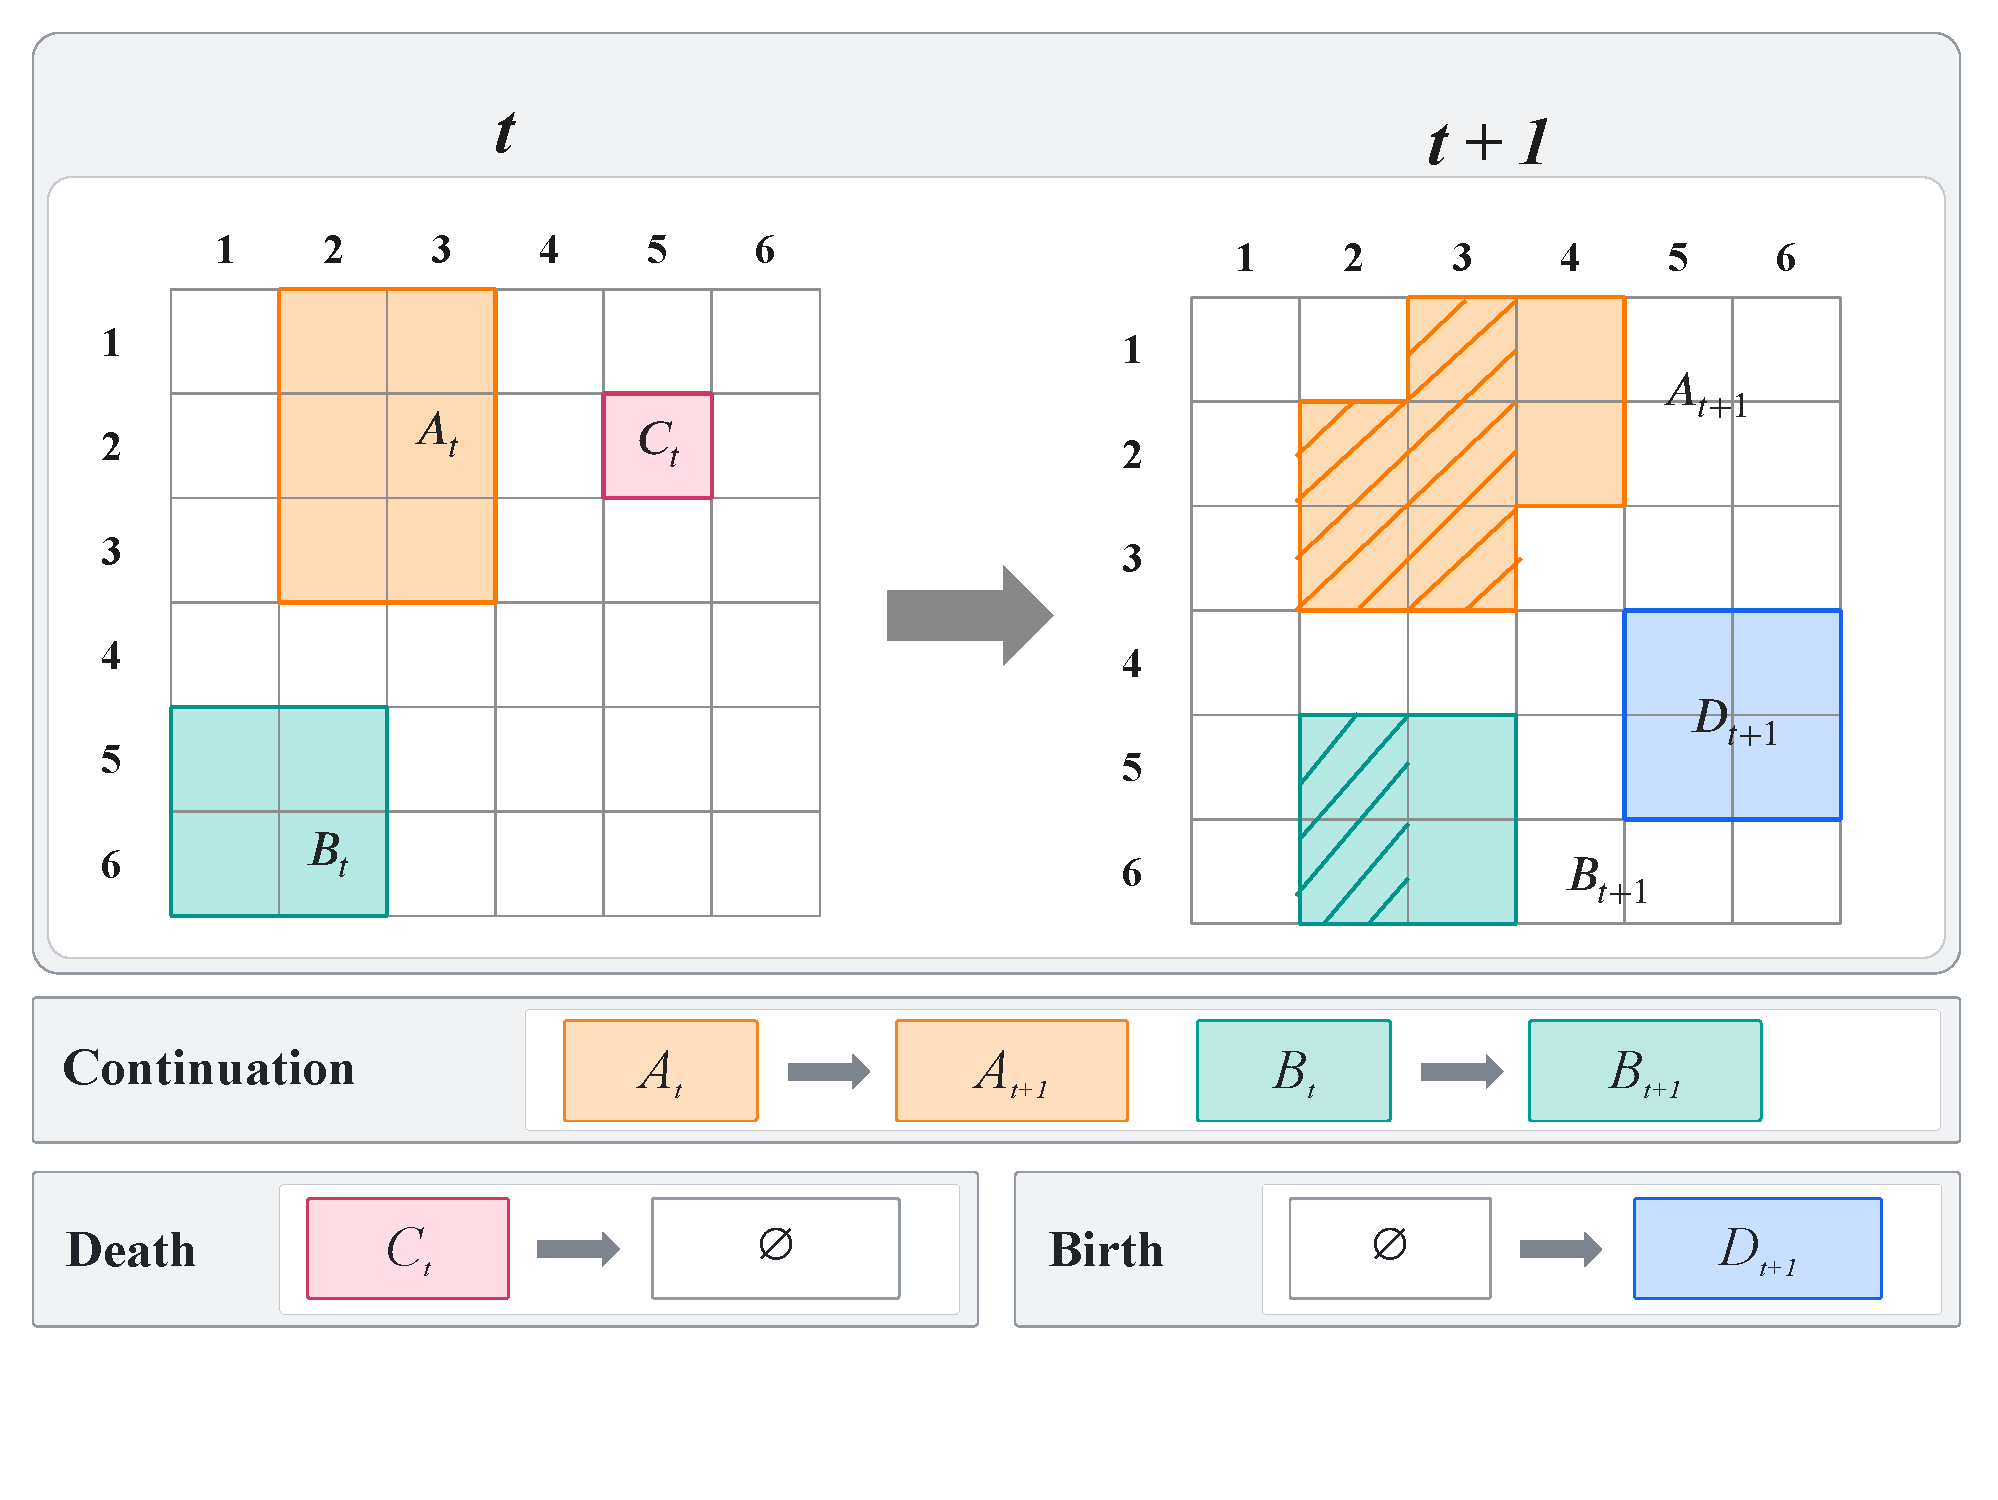
\includegraphics[width=\linewidth]{figures/anchor_leaf_correspondence.pdf}
\caption{Overlap-based leaf correspondence on a shared grid. Colored regions represent leaf-arc supports; hatching marks samples shared with the previous frame. Maximum-overlap one-to-one assignment continues $A$ and $B$, leaves $C_t$ unmatched, and assigns a new identity to $D_{t+1}$. Birth and death denote matching states, not identified physical events.}
\label{fig:leaf_correspondence}
\end{figure}

These correspondences, computed before any topology-budget sweep, provide the motion samples for Spatial Anchoring, which distinguishes a reference target $q_i^t$ from the display anchor $x_i^t$. Only valid consecutive-frame matches contribute displacements; failed matches or interrupted tracks contribute no sample for that step. By default, one unit direction $a^*\in\mathbb{R}^d$, $d\in\{2,3\}$, is estimated offline from all matched consecutive-frame extremum displacements:
\begin{equation}\label{eq:autodirection}
\begin{aligned}
 \Delta p_i^t&=p_i^t-p_{\mu_t(i)}^{t-1},\\
 S&=\sum_{t,i\;\mathrm{matched}}\Delta p_i^t(\Delta p_i^t)^\top,\\
 a^*&\in\arg\max_{\|a\|=1}a^\top Sa.
\end{aligned}
\end{equation}
The leading eigenvector maximizes squared projected motion, not feature count or topological compatibility. The same calculation serves 2D and 3D; it is performed once for the whole sequence. Its sign makes total signed projected motion nonnegative; for near-zero signed motion, the largest-magnitude component is made positive. With negligible motion energy, the longest domain axis is used (first axis on a tie). Repeated leading eigenvalues leave the maximizing direction nonunique; the reported eigengap indicates this ambiguity. A supplied physical direction may replace $a^*$ without changing the layout. Overlap matching may miss fast-moving features or those with changing or weakly overlapping supports, affecting the displacement sample and hence the estimated direction.

For the selected direction, the minimum and span of the projected domain bounding-box corners define a common origin $o$ and extent $L>0$. The reference is
\begin{equation}\label{eq:reference}
 q_i^t=\langle a^*,p_i^t\rangle-o\in[0,L].
\end{equation}
Direction, origin and scale remain fixed across frames and all budgets for the same prepared sequence. Implementation arrays store raw projections on $[o,o+L]$; translating both references and layout coordinates by $-o$ gives the paper convention. The origin is subtracted once, not again by the solver. Distinct extrema can share projected coordinates while retaining separate identities. Anchoring minimizes constrained deviation rather than requiring $x_i^t=q_i^t$.

Relative geometry uses distances $d_{ij}^t$ between leaf-support centroids. These differ from extremum references because a changing support can move its centroid while the extremum stays fixed. The automatic-reference adapter supplies extrema explicitly; the low-level solver also accepts precomputed references and otherwise defaults to centroid projection. Widths $W_i^t=s\,m_i^t$ convert positive support measures with a fixed scale $s$, without per-frame normalization.

With correspondence and the reference fixed, a frame comprises a leaf order, extremum anchors, and a scalar profile:
\begin{equation}\label{eq:mapframe}
 M_t=(\pi_t,x_t,\psi_t),\qquad\psi_t:[0,L]\to\mathbb{R}.
\end{equation}
We seek reference-aligned positions and motion while approximating relative geometry and controlling displayed topology. The interval-layout set $\mathcal{L}(\pi)$ requires intervals of widths $W_i$ centered at $z_i$ to lie inside the canvas, remain disjoint with gap at least $g\ge0$, and contain anchors satisfying $|x_i-z_i|\le\rho W_i/2$, $0\le\rho\le1$. Infeasible total widths and gaps are reported rather than rescaled.

Actual displacement is $|x_i-q_i|$, normalized by $L$ when reported. To distinguish order conflict from finite-width placement, define
\begin{equation}\label{eq:nroe}
 \nroe(\pi)=\frac{1}{2L}\max_{j\le k}
                      [q_{\pi(j)}-q_{\pi(k)}]^+.
\end{equation}
This is the smallest worst displacement of a nondecreasing point placement, divided by $L$; it ignores widths. For finite intervals, the exact fixed-order cost is
\begin{equation}\label{eq:tau}
 \tau(\pi)=\min_{(x,z)\in\mathcal{L}(\pi)}\|x-q\|_\infty.
\end{equation}
The minimum is attained whenever the layout set is nonempty. It is evaluated exactly from the fixed-order packing constraints, equivalently through a minimax linear program.

For distinct labels, let $V_{ij}^{\psi}$ be the maximum profile value between their anchors, with $V_{ii}^{\psi}=\psi(x_i)$. We require
\begin{equation}\label{eq:dtop}
\begin{aligned}
 \dtop(\psi_t,T_t)&=\max_{i,j}|V_{ij}^{\psi_t}-V_{ij}^t|\le\eta,\\
 \eta&=(\varepsilon_0+\varepsilon)\Delta_F.
\end{aligned}
\end{equation}
Here $\Delta_F>0$ is the sequence-wide scalar range, $\varepsilon_0$ is a fixed numerical allowance, and $\varepsilon\ge0$ is the sole primary user control. The implementation defaults to $\varepsilon_0=10^{-7}$. There is no 20\% cap: 100\% is neither a mathematical upper bound nor necessarily unrestricted topology. NMLE reports the achieved normalized error $\dtop/\Delta_F$. Exact topology means zero labelled error on the declared tree. A nonzero tie allowance is accounted for in $\eta$.

All remaining settings belong to a fixed configuration $\Theta_0$: position slack $\beta_0$, the four objective weights, width scale, gap, anchor slack and output resolution. For a prepared sequence, the default interface is $M_t^\varepsilon=\operatorname{AnchorMTM}(T_t,q_t,W_t,V_t,\mu_t;\varepsilon,\Theta_0)$. Advanced settings may be supplied once, but only $\varepsilon$ varies in a budget sweep. Supplementary Material specifies the fixed scale rules and implementation tolerances.

For canonical cophenetic merge-tree representations whose fixed labels cover every leaf and whose induced matrices include the diagonal, $\dtop$ equals the unnormalized labelled interleaving distance~\cite{Munch:2019:LINF,Gasparovic:2024:IID}. Under these conditions, $d_B\le d_I\le\dtop$~\cite{Morozov:2013:IDMT}. Unlabelled extrema introduced by rendering must be checked before applying this interpretation to the whole displayed tree.

\subsection{Spatially Anchored Layout Construction}\label{sec:construction}
With features and their reference fixed, construction chooses an order by the lexicographic objective
\begin{equation}\label{eq:orderobjective}
\begin{aligned}
 \pi_t^\varepsilon&\in\underset{\pi\in\mathcal{C}_t(\varepsilon)}{\arg\min}
                    \bigl(\tau_t(\pi),\nroe_t(\pi)\bigr),\\
 &\hspace{1em}\mathrm{s.t.}\quad\delta_t^*(\pi)\le\eta(\varepsilon).
\end{aligned}
\end{equation}
The finite candidate pool contains the original strict-topology order, midpoint initializations, and orders visited during width-aware refinement of threshold and selective flattenings. Every candidate is evaluated against the same source merge matrix. Selection minimizes $\tau$ first and NROE second; it is not a global optimum over all permutations. Algorithm~\ref{alg:construction} separates this discrete selection from fixed-order placement.

\begin{algorithm}[htbp]
\caption{Single-Control AnchorMTM}\label{alg:construction}
\KwData{2D/3D field sequence and grid; $\varepsilon\ge0$; fixed configuration $\Theta_0$.}
\KwResult{Temporal map $I^\varepsilon$, error records, or a failure report.}
Extract augmented trees, leaf supports and extrema; match supports and assign Track IDs\;
Estimate one direction and fixed references $q_t$; reuse this preprocessing across budgets\;
$\eta\leftarrow(\varepsilon_0+\varepsilon)\Delta_F$\;
\For{each time step $t$ in temporal order}{
 Report and stop if widths and gaps exceed the fixed canvas\;
 $\mathcal{C}_t\leftarrow\operatorname{GenerateAndRefine}(T_t,q_t,W_t,V_t,\eta)$; retain strict-topology candidates\;
 Evaluate $\tau(\pi)$, $\nroe(\pi)$ and $\delta^*(\pi)$ for candidates\;
 $\mathcal{F}_t\leftarrow\{\pi\in\mathcal{C}_t:\delta^*(\pi)\le\eta\}$\;
 \lIf{$\mathcal{F}_t=\varnothing$}{report no feasible candidate and stop}
 Select $\pi_t^\varepsilon$ from $\mathcal{F}_t$ by $(\tau,\nroe)$\;
 Compute optimal merge barriers for $\pi_t^\varepsilon$\;
 Solve the four-term QP only for $\pi_t^\varepsilon$, with cap $\tau(\pi_t^\varepsilon)+\beta_0$ and valid matched history\;
 Reconstruct the profile by leaf/LCA filling and barrier correction\;
 Record candidate counts, continuous and rendered errors, motion and failures; append profile to $I^\varepsilon$\;
}
\KwReturn{$I^\varepsilon$ and diagnostic records}\;
\end{algorithm}

\subsubsection{Topology-Budgeted Leaf Ordering}
\emph{Exact Mode} sets $\eta=0$ and requires zero labelled merge error on the supplied tree. \emph{Budgeted Mode} permits $\eta>0$. Setting only the additional budget $\varepsilon=0$ while retaining $\varepsilon_0>0$ gives a numerical allowance, not zero labelled error. Both modes share the same interval model and placement objective.

Candidate generation includes the exact tree, threshold flattenings, and a conflict-driven selective flattening. Midpoint orders initialize these structures. Width-aware block insertion refines the four best initial structures, together with the exact tree, while retaining the point-model budget order as a candidate. Moves improve the lexicographic score consisting of $\tau$ and a squared packing-residual term, and must pass $\delta^*(\pi)\le\eta$. Visited initial and trial orders are retained in the deduplicated pool, including the strict-tree initialization and retained point candidate. Final budget filtering and lexicographic selection use the exact fixed-order costs; refinement does not certify a global optimum over permutations. 

Helpers inherit the current geometry and layout parameters. Comparisons use the implementation's numerical tolerances. The guards report capacity failure or an empty admitted set; no widths, gaps or canvas scales are silently changed. The exact-tree structure is always retained among refinement seeds, and its child-block moves preserve strict topology in the exact model. Its presence does not guarantee successful numerical placement or raster reconstruction; capacity, input and solver failures remain possible. An empty admitted set is never selected from. Invalid input and numerical solver failures propagate as errors, separately from mathematical infeasibility. First-frame and unmatched history contributes no temporal target.

\subsubsection{Optimal Merge Barriers and Topological Feasibility}
For a fixed order, a pair's displayed merge is the largest intervening barrier. Set $C_k=\min_{i\le k<j}V_{\pi(i)\pi(j)}$ and $F_k=\max(V_{\pi(k)\pi(k)},V_{\pi(k+1)\pi(k+1)})$ for gap $k$.
\begin{proposition}[Optimal barriers]\label{prop:barriers}
With fixed extremum values in the continuous non-strict model, the smallest labelled merge error is
\begin{equation}\label{eq:delta}
\begin{split}
 \delta^*(\pi)=\max\bigg\{&0,\max_k(F_k-C_k),\\
 &\frac12\max_{i<j}\left(V_{\pi(i)\pi(j)}-
                         \max_{i\le k<j}C_k\right)\bigg\},
\end{split}
\end{equation}
and barriers $b_k=C_k+\delta^*(\pi)$ attain it.
\end{proposition}
Error $\delta$ requires $F_k\le b_k\le C_k+\delta$. Choosing the largest admissible barriers satisfies every pair's lower merge requirement exactly when $\delta\ge\delta^*$. Thus the order meets the merge-level allowance in this continuous model exactly when $\delta^*(\pi)\le\eta$. This fixed-order test supports candidate search without making it globally optimal. Strict-extremum clearance and raster effects are checked separately.

\subsubsection{Spatially Anchored Spatiotemporal Placement}
Once the order is fixed, the core terms are $E_R$, mean squared deviation from the fixed reference, and $E_M$, mean squared error in matched projected motion. The auxiliary term $E_G$ approximates support-centroid distances through ordered anchor separations; $E_C$ regularizes anchor offsets from interval centers. All four terms and their nonnegative weights are retained:
\begin{equation}\label{eq:qp}
\begin{aligned}
 \min_{x_t,z_t}\quad&\lambda_R E_R+\lambda_G E_G+\lambda_M E_M+\lambda_C E_C\\
 \mathrm{s.t.}\quad&(x_t,z_t)\in\mathcal{L}(\pi_t),\\
 &\|x_t-q_t\|_\infty\le\tau(\pi_t)+\beta_0.
\end{aligned}
\end{equation}
For each valid match, set $\Delta q_i^t=q_i^t-q_{\mu_t(i)}^{t-1}$ and use the previous display anchor plus this reference displacement as the temporal target:
\begin{equation}\label{eq:temporal_target}
 \hat x_i^t=x_{\mu_t(i)}^{t-1}+(q_i^t-q_{\mu_t(i)}^{t-1}).
\end{equation}
Thus $E_M$ follows projected motion while favoring continuity of $x-q$. First-frame, newly born and otherwise unmatched leaves have no previous-frame motion penalty. Each term is averaged over its features, ordered pairs or valid matches; the current automatic-reference adapter uses unit confidence for valid matches. Supplementary Material distinguishes this default from legacy confidence-weighted paths.

Only $\varepsilon$ changes the topology allowance $\eta(\varepsilon)$. The fixed slack $\beta_0\ge0$ bounds additional position deviation after ordering. The cap is feasible because $\tau(\pi_t)$ is attained; the QP receives only the selected order and cannot replace it by one with a lower quadratic objective. It bounds continuous displacement while geometry and temporal objectives select a compromise within that cap. The fixed-order problem is convex; sequential processing does not imply a joint sequence optimum or exact preservation of every projected motion.

\subsubsection{Profile Reconstruction and Output Diagnostics}
Reconstruction inherits the leaf-arc sampling and LCA-path filling of the merge tree map pipeline~\cite{Koepp:2023:TMTM,STMTM:2026}. Original extrema remain at their anchors; regular samples provide scalar context within intervals and gaps. Optimal-barrier correction then clips each inter-anchor interior to $b_k$ and raises an existing peak if necessary. This separate correction is required for relaxed orders; inherited LCA filling alone does not enforce the minimax barriers.

A common direction, origin, extent, and pixel conversion are used for all frames. The profiles form the final temporal map,
\begin{equation}\label{eq:map}
 I^\varepsilon(t,u)=\psi_t^\varepsilon(u),\qquad 0\le u\le L.
\end{equation}
There is no per-frame recentering. Resampling does not retain every source sample, and corrected interior values need not remain in the original scalar range. Strict-extremum clearance and raster rounding can change the achieved error. Raster-capacity and nonfinite-value errors stop reconstruction; the existing optimal-filling analysis records measured budget deviations and topology diagnostics without automatic repair or a universal rejection gate. Full-tree interpretation additionally requires checking label coverage. A recorded profile is therefore not unconditionally certified by $\delta^*\le\eta$. Records distinguish the requested budget, position certificates, attained $\tau$, continuous $\delta^*$, and actual rendered errors. 

\subsection{Certified Position--Topology Bounds}\label{sec:bounds}
The construction can leave reference displacement even after optimization. The following bounds explain what topology and finite widths make unavoidable: the first answers how much a tree-compatible point order must deviate, the second adds interval packing, and the third asks which restrictions survive a merge-error allowance. They are analytical benchmarks, not three execution stages or search-pruning rules; construction uses the exact fixed-order costs $\tau$ and $\delta^*$. The resulting certificates apply independently of the layout algorithm. Full proofs and computational definitions accompany the paper in Supplementary Material. We suppress $t$ within a frame, use $[v]^+=\max(v,0)$, and take empty maxima as zero.

\subsubsection{Exact-Topology Reference-Order Bound}
For a reduced tree with strictly increasing proper-ancestor levels, exact topology makes every subtree contiguous. Let $[m_X,M_X]$ be the reference hull of the leaves in subtree $X$.
\begin{theorem}[Exact-Topology Position Bound]\label{thm:order}
Every zero-error profile has $\nroe(\pi)\ge\nu^*(T,q)$, where
\begin{equation}\label{eq:nu}
 \nu^*(T,q)=\frac{1}{2L}\max_v\max_{\substack{X,Y\in\mathrm{ch}(v)\\X\ne Y}}
 [\min(M_X-m_Y,M_Y-m_X)]^+.
\end{equation}
Recursive child ordering by reference-hull midpoint attains this point-model order bound in $O(n\log n)$ time.
\end{theorem}
\begin{proof}[Proof sketch]
Sibling blocks must choose one orientation. Their two possible inversion costs are $[M_X-m_Y]^+/2$ and $[M_Y-m_X]^+/2$. Midpoint order chooses the smaller; every inverted leaf pair is separated by sibling blocks at its LCA.
\end{proof}
This result isolates the ordering restriction imposed by the tree and references. Midpoint ordering attains the point-order optimum; finite intervals introduce additional constraints, considered next.

\subsubsection{Width-Aware Position Bound}
Finite widths, minimum gaps, anchor slack and canvas capacity add packing costs to the point-order obstruction. For a nonempty leaf set $S$, let $H_i=\rho W_i/2$, $\ell_i=q_i-W_i/2-H_i$, $h_i=q_i+W_i/2+H_i$, and $s_i=W_i+g$. Define two packing summaries:
\begin{equation}\label{eq:packing}
\begin{aligned}
 A(S)&=\max_{a\in S}\left(\ell_a+\sum_{\substack{i\in S\\\ell_i\ge\ell_a}}s_i\right),\\
 B(S)&=\max_{b\in S}\left(\sum_{\substack{i\in S\\h_i\le h_b}}s_i-h_b\right).
\end{aligned}
\end{equation}
The first uses upper reference-endpoint sets and the second lower sets; sorting and cumulative sums evaluate them. For disjoint leaf sets $X,Y$ and the full leaf set $\mathcal{F}$, write
\begin{equation}\label{eq:packingcost}
\begin{aligned}
 \omega(X,Y)&=\tfrac12\min\{A(X)+B(Y),A(Y)+B(X)\}-\tfrac g2,\\
 E_\partial&=\max\{0,B(\mathcal{F})-g,A(\mathcal{F})-g-L\}.
\end{aligned}
\end{equation}
Here $\omega$ takes the cheaper block orientation and $E_\partial$ accounts for both canvas ends. Let $\mathcal{P}_0$ contain every pair of distinct sibling descendant-leaf sets. The certificate is
\begin{equation}\label{eq:bwdef}
 \mathcal{B}_w(T,q,W)=\max\{E_\partial,\max_{(X,Y)\in\mathcal{P}_0}\omega(X,Y)\}.
\end{equation}
The dependence on $g$, $\rho$ and $L$ is through Eqs.~\ref{eq:packing}--\ref{eq:packingcost}; it is suppressed in the certificate's arguments.
\begin{theorem}[Width-Aware Position Bound]\label{thm:width}
For any feasible exact-topology interval layout,
\begin{equation}\label{eq:widthbound}
 \|x-q\|_\infty\ge\tau(\pi)\ge\mathcal{B}_w(T,q,W).
\end{equation}
With zero widths and gaps, $\mathcal{B}_w=L\nu^*(T,q)$.
\end{theorem}
\begin{proof}[Proof sketch]
The first and last anchors of selected leaves must enclose their intervals and intervening gaps, up to the allowed anchor slack. Upper and lower sets in Eq.~\ref{eq:packing} maximize the resulting shortfall against reference separation. Exact topology requires one orientation of every sibling pair; the canvas ends give the two one-sided costs.
\end{proof}
Thus $\mathcal{B}_w$ bounds all exact-topology legal interval orders and need not be attained; $\tau(\pi)$ is the attained minimum for a specified order. These quantities have coordinate units, whereas NROE and $\nu^*$ are normalized by $L$.

\subsubsection{Bounded-Topology Position Bound}
A merge-level allowance can release some contiguous blocks, but still limits interleaving. If leaf $k$ lies between descendants $i,j$ of node $u$, interval containment gives $V_{ik}^{\psi}\le V_{ij}^{\psi}$, hence $V_{ik}\le h(u)+2\eta$. Define $A_\eta(u)$ as the highest ancestor, including $u$, with $h(A_\eta(u))-h(u)\le2\eta$. This uses the accumulated ancestor-height difference in scalar units, on the reduced equal-level tree with the fixed labels of Eq.~\ref{eq:dtop}.

Let $\mathcal{P}_\eta$ consist of two types of leaf-set pairs: $(\mathcal{D}(u),\{k\})$ for every internal node $u$ and leaf $k\notin\mathcal{D}(A_\eta(u))$; and $(\mathcal{D}(u),\mathcal{D}(w))$ for internal nodes $u,w$ satisfying
\begin{equation}\label{eq:separatedpairs}
\begin{aligned}
 \mathcal{D}(w)\cap\mathcal{D}(A_\eta(u))&=\varnothing,\\
 \mathcal{D}(u)\cap\mathcal{D}(A_\eta(w))&=\varnothing.
\end{aligned}
\end{equation}
For any nonempty leaf set $X$, use its reference hull $[m_X,M_X]$ and define $\kappa(X,Y)=[\min(M_X-m_Y,M_Y-m_X)]^+/(2L)$. The two certificates are
\begin{equation}\label{eq:chaindef}
\begin{aligned}
 C_\eta(T,q)&=\max_{(X,Y)\in\mathcal{P}_\eta}\kappa(X,Y),\\
 C_{w,\eta}(T,q,W)&=\max\{E_\partial,\max_{(X,Y)\in\mathcal{P}_\eta}\omega(X,Y)\}.
\end{aligned}
\end{equation}
\begin{theorem}[Bounded-Topology Position Bound]\label{thm:chain}
In a profile with $\dtop\le\eta$, no leaf outside $\mathcal{D}(A_\eta(u))$ can lie between two leaves of $u$. Every pair in $\mathcal{P}_\eta$ lies wholly in one block orientation or the other. Consequently,
\begin{equation}\label{eq:chainbounds}
 \nroe(\pi)\ge C_\eta(T,q),\qquad
 \tau(\pi)\ge C_{w,\eta}(T,q,W),
\end{equation}
with the second inequality applying to the interval model.
\end{theorem}
The separation principle excludes interleaving for each eligible pair; the two possible orientations then yield $\kappa$ and $\omega$. Thus $C_\eta$ bounds normalized reference-order error, while $C_{w,\eta}$ includes finite-width and boundary costs in coordinate units. Accumulated ancestor gaps make these certificates at least as strong as those obtained by flattening every parent gap at most $2\eta$.

The allowance concerns the displayed hierarchy; the source field and feature identities stay fixed. A larger feasible set need not improve every feature or every heuristic result. These bounds are reported as benchmarks for unavoidable error; ranking and continuous acceptance use the exact fixed-order evaluations in Section~\ref{sec:construction}. Continuous feasibility does not certify the full rendered raster.

\section{Experiments}\label{sec:experiments}
The experiments ask how far existing merge tree maps lie from a spatial reference and how much of this distance topology forces (Section~\ref{sec:compare}), how tight the three bounds are and what a merge-level budget buys (Section~\ref{sec:tradeoff}), what the maps show on real data (Section~\ref{sec:cases}), and which components matter at what cost (Section~\ref{sec:ablation}).

\subsection{Experimental Setup}\label{sec:setup}
\paragraph{Data.} Table~\ref{tab:data} lists seven sequences with 917 frames: five planar fields from reanalysis, satellite, emission and air-quality records and one synthetic control, and two volumetric flow simulations~\cite{Hersbach:2020:ERA5,Franke:2021:1DP,NOAA:OLR,Dong:2026:PM25,Koepp:2023:TMTM,Popinet:2004:Tangaroa,Camarri:2005:Cylinder,Weinkauf:SquareCylinder}. All methods share the processed fields, augmented trees, leaf supports, correspondences and references. Two further sequences serve only as illustrations and are excluded from all aggregates: the 744 hourly Storms frames of Figure~\ref{fig:storms_overview} and a 90-frame volumetric Vortex sequence.

\begin{table}[t]
\caption{Benchmark sequences. Leaves: retained extrema per frame.}\label{tab:data}
\centering\scriptsize\setlength{\tabcolsep}{3pt}
\begin{tabular}{llrrl}\toprule
Sequence & Scalar field & Frames & Leaves & Tree\\\midrule
Storms & ERA5 mean sea-level pressure, 2D & 118 & 1--8 & join\\
Wildfires & $\log(1+\mathrm{FRP})$, 2D & 30 & 6--11 & split\\
OLR & outgoing longwave radiation, 2D & 60 & 2--8 & join\\
PM$_{2.5}$ & PM$_{2.5}$ concentration, 2D & 366 & 1--7 & split\\
Ring & synthetic ring intensity, 2D & 40 & 1--7 & split\\
Tangaroa & velocity magnitude, 3D & 201 & 18--93 & join\\
Cylinder & Q criterion, 3D & 102 & 4--75 & split\\\bottomrule
\end{tabular}
\end{table}

\paragraph{Methods.} We compare the native outputs of TMTM~\cite{Koepp:2023:TMTM} and ST-MTM~\cite{STMTM:2026}; an earlier threshold construction ($\kappa$) that flattens every merge with parent gap below $20\%$ of $\Delta_F$ and places anchors by a quadratic program without a merge-error cap; a projection baseline ($\varepsilon=\infty$) that sorts every frame by $q$ and uses the same optimal barriers and capped QP as ours; and AnchorMTM in Exact Mode ($\varepsilon=0$) and Budgeted Mode ($\varepsilon=10\%$ unless stated), with $\varepsilon_0=10^{-7}$ and one fixed configuration $\Theta_0$ for all sequences. Given their native leaf orders, our implementation reproduces both previous layouts on all planar sequences: the TMTM linearization matches the official implementation in all 3127 arc intervals and anchors, and the ST-MTM anchors satisfy the optimality conditions of its quadratic programs (relative KKT residuals below $10^{-6}$). Both previous methods are heuristic in the leaf order: ST-MTM's order exceeds the exhaustive optimum of its own objective on 10 frames, and TMTM's greedy choice is optimal at 434 of 463 enumerated steps but up to 85.5\% above the per-step optimum elsewhere.

\paragraph{Metrics.} Position is measured by NROE (Eq.~\ref{eq:nroe}), which compares methods with different native scales by order alone, and, for layouts that share our interval model, by the pooled mean $E_{\mathrm{pool}}$ and worst $E_\infty$ of $|x_i-q_i|/L$ over all feature--frames. Topology is measured by NMLE, the rendered $\dtop/\Delta_F$ (Eq.~\ref{eq:dtop}), as worst and mean over frames. Following the protocol of ST-MTM~\cite{STMTM:2026}, we also report scale-normalized stress (SNS) and trustworthiness (TW, $k=1$) of anchor distances against support-centroid distances. The motion error (ME) is the fraction of clear approach or separation events between two matched features over two steps that the map shows in the wrong direction or not at all. Recomputing the stored baseline values from their saved anchors reproduces SNS to a relative $10^{-5}$ and TW and ME to the third decimal or one event.

\subsection{Quantitative Comparison}\label{sec:compare}
\begin{figure*}[t]
\centering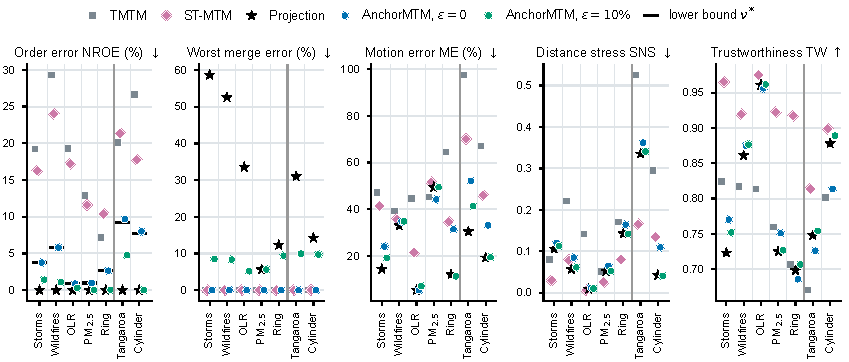
\includegraphics[width=\linewidth]{figures/fig_compare.pdf}
\caption{Comparison on seven sequences (left of the grey line: planar; right: volumetric). Order error NROE with the exact-topology lower bound $\nu^*$ of Theorem~\ref{thm:order} (black ticks), worst merge error, motion error, and the two distance measures of ST-MTM. Exact-topology methods (TMTM, ST-MTM, AnchorMTM at $\varepsilon=0$) have zero merge error; the projection has zero order error but up to 59\% merge error. All values are listed in the supplement.}\label{fig:compare}
\end{figure*}

Figure~\ref{fig:compare} compares all methods. \emph{Order.} By Theorem~\ref{thm:order}, no exact-topology output can fall below $\nu^*$; what differs between methods is the excess above it. Most of the order error of TMTM and ST-MTM is such excess: on Storms, TMTM's 19.2\% contains 3.8\% that the hierarchy forces, and ST-MTM's 16.3\% contains 12.5\% that it does not. Exact Mode lies within 0.03 percentage points of $\nu^*$ on every planar sequence. On Tangaroa and Cylinder, the width-aware search trades a little NROE (9.67\% against 9.24\% on Tangaroa) for a lower worst displacement (Section~\ref{sec:ablation}).
\emph{Topology.} The projection has zero order error but changes merge levels by up to 58.66\% of the scalar range on Storms, 52.58\% on Wildfires, 33.56\% on OLR and 31.02\% on Tangaroa, where no frame keeps its tree; the uncapped $\kappa$ construction reaches the same worst values on OLR and Tangaroa. No Budgeted Mode map exceeds its budget.
\emph{Motion.} Exact Mode makes fewer motion errors than both TMTM and ST-MTM on all seven sequences, e.g., 5.4\% against 21.4\% on OLR and 52.2\% against 70.0\% on Tangaroa, because a feature that moves along the reference also moves on the map. The projection, which follows the references exactly, has the lowest motion error on most sequences.
\emph{Distance.} ST-MTM, which optimizes pairwise distances, has the best TW on all seven sequences and the best SNS on five. Anchoring to one direction therefore trades two-dimensional distance preservation for position along that direction. On Cylinder, Budgeted Mode (SNS 0.041) and the $\kappa$ construction (0.040) are far below ST-MTM (0.135).

The supplement shows maps of OLR and Ring with the same renderer and widths. On Ring, the TMTM objective keeps all features near the centre of the axis and the ST-MTM objective spreads them by pairwise distance; both place them far from their references, whereas Exact Mode follows them and a 10\% budget changes the map only locally. On OLR, Exact Mode already places the low-radiation basins near their references, so the map reads like a time--longitude plot while keeping each basin's nesting.

\subsection{Certified Bounds and Position--Topology Trade-off}\label{sec:tradeoff}
\begin{figure}[t]
\centering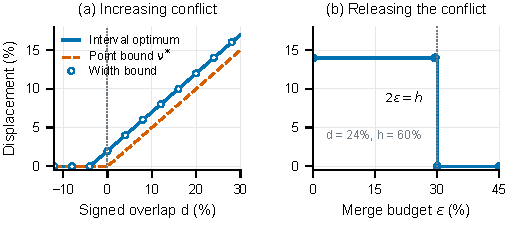
\includegraphics[width=\columnwidth]{figures/fig_controlled_conflict.pdf}
\caption{Controlled four-leaf trees. (a) Increasing sibling-hull overlap forces displacement; circles mark the width bound of Theorem~\ref{thm:width}, which the exhaustive interval optimum attains. (b) At overlap $d=24\%$, the $14\%$ interval displacement disappears only when the merge budget reaches half the parent gap $h=60\%$ (Theorem~\ref{thm:chain}). Percentages refer to a unit canvas or a unit scalar range.}\label{fig:controlled}
\end{figure}

\paragraph{Controlled conflict.} To isolate the conflict, we fix two sibling pairs $X=\{A,B\}$ and $Y=\{C,D\}$ that merge at $0.4$ below a root at $1$, with leaf values $0$. On a unit canvas their references are $(0.2,0.5,0.5-d,0.8-d)$, with signed overlap $d$ from $-0.12$ to $0.30$. Across 43 overlaps and four widths, we enumerate all 24 leaf orders and solve independent minimax placement LPs. The point optimum is exactly $\nu^*=\max(0,d)/2$. With equal widths $W=0.06$, gap $0.01$ and $\rho=0.5$, both the width bound and our search attain the exhaustive optimum $\tau=\max(0,(d+0.04)/2)$ (Fig.~\ref{fig:controlled}a); at $d=0.24$ the point and interval costs are 12\% and 14\%. Sweeping the budget for four parent gaps confirms that interleaving becomes admissible at $2\varepsilon=h$: for $h=0.6$, displacement vanishes at $\varepsilon=0.3$ (Fig.~\ref{fig:controlled}b). These are controlled instances, not a general tightness claim for the width bound.

\begin{figure*}[t]
\centering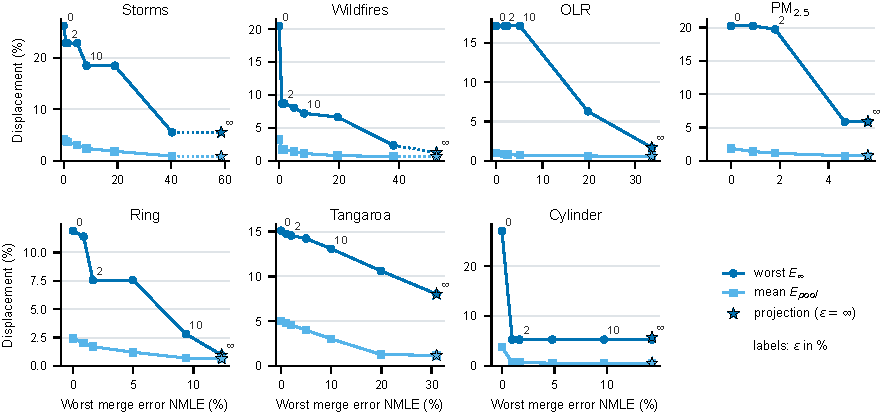
\includegraphics[width=\linewidth]{figures/fig_frontier.pdf}
\caption{Position--topology trade-off per sequence. Each point is one layout of all frames at budget $\varepsilon$ (labels, in percent), placed by its rendered worst merge error and its worst (dark) and mean (light) displacement. Stars: projection ($\varepsilon=\infty$). Grey crosses: the uncapped $\kappa$ construction, planar sequences only.}\label{fig:frontier}
\end{figure*}

\paragraph{Trade-off.} Figure~\ref{fig:frontier} places every layout by its rendered worst merge error and its displacement, from Exact Mode to the projection. On Cylinder, a 1\% budget reaches the lowest worst displacement of the whole curve (27.00\% to 5.27\%), below the projection's 5.73\%, because sorting by reference ignores widths. On Wildfires, 1\% reduces $E_\infty$ from 20.48\% to 8.71\%, and on PM$_{2.5}$ 5\% reaches the projection result. Storms needs much more: its worst displacement stays above 18\% up to $\varepsilon=20\%$, and OLR keeps $E_\infty=17.14\%$ up to 10\% because one frame needs a larger change. Mean merge errors are far below the maxima (Storms at 10\%: 0.90\% mean, 8.51\% worst), so the budget is spent on few frames. At similar positions, the declared budget now bounds the worst merge error, which the uncapped $\kappa$ construction does not (Storms: 26.07\% to 8.51\%; Wildfires: 19.56\% to 8.35\%).

\paragraph{Local budget response.} Aggregate gains do not imply pointwise improvement. In a four-leaf control, enumerating all 24 orders lowers the optimal worst displacement from 22\% to 1\% at $\varepsilon=30\%$, yet one feature's error rises from 0.087\% to 1\%. On the Vortex diagnostic, increasing $\varepsilon$ from 20\% to 30\% lowers the pooled error from 8.79\% to 4.27\%, while 30.91\% of 12{,}446 feature--frame observations worsen, 24.72\% by at least 0.5 percentage points of $L$. The supplement gives the fixed-population protocol.

\paragraph{Tightness on large trees.} Theorem~\ref{thm:order} is attained exactly by midpoint ordering. The width bound is attained on most planar frames and on the worst Tangaroa and Cylinder frames, but not uniformly. The bounded-topology bound keeps the certificates informative on large trees: on Tangaroa at $\varepsilon=5\%$, flattening every gap below $2\eta$ gives a bound of only 0.38\% on average, whereas Theorem~\ref{thm:chain} with widths gives 7.40\% against an attained 8.10\%. A gap of about one percentage point also remains at $\varepsilon=0$, which suggests that the bound, not the search, is loose there. On Wildfires at $\varepsilon>0$ and on one OLR frame at $\varepsilon=10\%$, a worst-frame gap remains.

\begin{figure*}[t]
\centering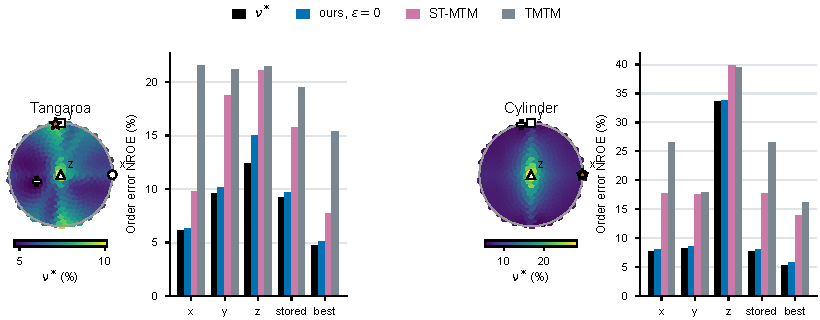
\includegraphics[width=\linewidth]{figures/fig_direction.pdf}
\caption{Reference direction in 3D. Disks: mean order bound $\nu^*$ over 400 directions of the hemisphere (equal-area projection; centre $=z$, rim $=xy$ plane); markers: coordinate axes, the automatically estimated direction (star) and the smallest bound (cross). Bars: $\nu^*$ and mean order error of Exact Mode, ST-MTM and TMTM for the key directions (native orientations chosen in their favour).}\label{fig:direction}
\end{figure*}

\paragraph{Reference direction in 3D.} Projecting a volume onto one direction discards two coordinates, so the unavoidable order error depends on the direction. Because the bounds need only the tree and the extremum positions, we recomputed them for 400 directions over the hemisphere on both volumetric sequences, with references built as in Eq.~\ref{eq:reference} (Fig.~\ref{fig:direction}). The bound varies widely: its mean ranges from 4.70\% to 10.14\% on Tangaroa and from 5.26\% to 28.15\% on Cylinder. On Tangaroa, the estimated motion direction is among the most costly: only 3 of the 400 directions have a higher bound, and the $x$ axis would lower $\nu^*$ from 9.24\% to 6.09\%. On Cylinder, the streamwise axis lies near the median (7.72\%). In every key direction the previous methods stay far above the bound, while Exact Mode stays within 0.6 percentage points of it, except on the Tangaroa $z$ axis (2.6 points), where large widths dominate. Since $\nu^*$ costs milliseconds per frame, an analyst can compare candidate directions before computing any map and weigh following the motion against hierarchical conflict.

\subsection{Qualitative Case Studies}\label{sec:cases}
\paragraph{Storms.} On the 118-frame Storms benchmark, minima of sea-level pressure are low-pressure systems crossing the North Atlantic. Within the same layout model, the TMTM and ST-MTM objectives place features on average 37.3\% and 50.7\% of the canvas from their references in the worst case of each step. Exact Mode has a median of 0.8\% and a mean of 5.1\%, with peaks of up to 26.2\% in a few steps where the hierarchy conflicts with the reference. A 10\% budget lowers the mean to 2.7\%. It is spent in 31 of 118 steps, at most 8.51\% and 0.90\% on average, and the 89 barriers whose merge level changed by more than 0.1\% of the scalar range are marked on the map; at $\varepsilon=0$ no mark appears. Figure~\ref{fig:storms_overview} applies the same construction at $\varepsilon=5\%$ to 744 hourly pressure fields of December 1999. Five snapshots follow one matched minimum, a strong storm over Scandinavia, from 16 to 19 December. The leaf-arc supports outlined in the snapshots are the objects that the correspondence of Section~\ref{sec:method} matches, and the dashed guides show where each extremum appears in its profile. In the map, the displayed positions of this feature (blue) form one continuous track through the outlined window. The track is a computational correspondence of leaf features; it does not by itself establish physical storm genesis or dissipation.

\begin{figure*}[t]
\centering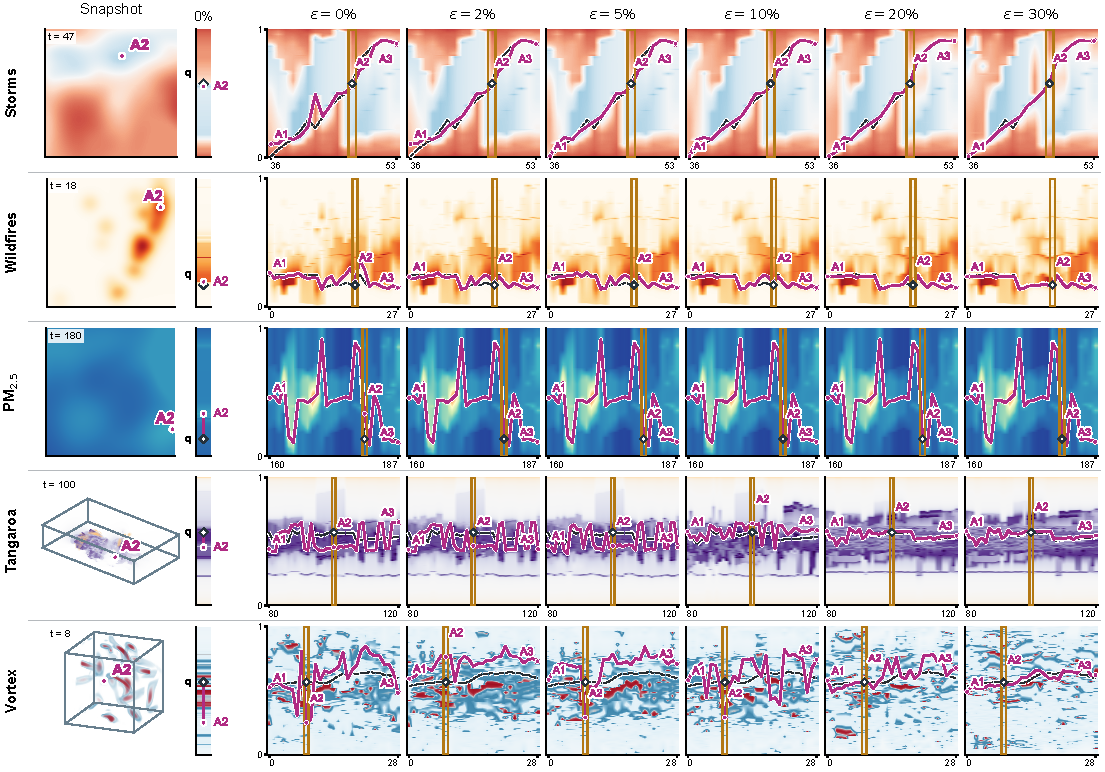
\includegraphics[width=\linewidth]{figures/fig_dataset_overview_extended.pdf}
\caption{Snapshots, Exact Mode strips and budget responses for Storms, Wildfires, PM$_{2.5}$, Tangaroa and Vortex. Each row shows the same tracked extremum at the window start (A1), snapshot time (A2) and window end (A3), across $\varepsilon=0,2,5,10,20,30\%$. Circles indicate mapped positions and diamonds spatial references; gold boxes select the snapshot profile column. Black dashed curves show the reference trajectory. Volume snapshots include their domain boxes; Tangaroa is non-cubic. Within each row all budgets share a colour scale; Tangaroa and Vortex use their volume-rendering transfer functions, and PM$_{2.5}$ uses a fixed [12,80] display range for the selected window.}\label{fig:datasetoverview}
\end{figure*}

\paragraph{Cross-dataset snapshots.} Figure~\ref{fig:datasetoverview} pairs spatial snapshots with 18--41 original time steps on three planar and two volumetric sequences. Each row keeps one input feature and its reference across all six budgets; A1--A3 index time samples, not different extrema. Four rows use benchmark inputs; the Vortex row is the separate diagnostic, whose reference $q=X/127$ is a normalized voxel coordinate because physical units are unavailable. The $30\%$ layouts were recomputed from the first frame through the end of each window, so they keep their temporal history, and all displayed windows satisfy their merge and position caps. The paired curves expose local shifts of individual features that the aggregate errors of Figure~\ref{fig:frontier} hide.

\subsection{Ablation Study and Performance}\label{sec:ablation}
\begin{table}[t]
\caption{Volumetric sequences (percent). $\kappa$ P (exact) and $\kappa$ R2 (relaxed, no merge-error cap) are the earlier threshold construction; N1 orders by NROE only; ours uses the width-aware search. Jump: mean $|\Delta x-\Delta q|/L$ of matched features.}\label{tab:volume}
\centering\scriptsize\setlength{\tabcolsep}{2.4pt}
\begin{tabular}{llrrrrr}\toprule
 & Layout & $E_{\mathrm{pool}}$ & $E_\infty$ & NROE & jump & NMLE max\\\midrule
\csname @@input\endcsname tables/tab_volume.tex
\bottomrule
\end{tabular}
\end{table}

\paragraph{Width-aware ordering.} Ordering for the point model is not enough when features are large. On Tangaroa, ordering by NROE alone (N1 in Table~\ref{tab:volume}) gives a worst displacement of 20.69\%, above the $\kappa$ construction's 16.86\%. Ranking candidates by the exact interval cost $\tau$ lowers it to 15.10\% at $\varepsilon=0$ and to 14.55\% at $\varepsilon=2\%$, where the worst frame meets the lower bound; on Cylinder, $\varepsilon\ge2\%$ lowers $E_\infty$ from 5.73\% to 5.27\%, again at the bound. The point-model order lies far above the bound in the first 30 Tangaroa steps, and the width-aware order removes most of this excess (supplement). The $\kappa$ construction keeps lower mean jumps on Tangaroa (2.59\% against 2.82\%) and a lower pooled displacement than our 2\% map (4.16\% against 4.55\%), but its merge error has no cap.

\paragraph{Search coverage and merge-error cap.} The candidate search is heuristic, so we checked it against exhaustive enumeration: on all 637 frames with at most eight leaves, the selected order matches the exhaustive optimum at nine budgets from 0 to 100\%. Removing the merge-error cap, i.e., the $\kappa$ construction, reaches similar positions with up to three times the worst merge error (Section~\ref{sec:tradeoff}).

\paragraph{Performance.} The bounds cost $O(n\log n)$ to $O(n^2\log n)$ and $\delta^*$ costs $O(n^3)$ per order. On an Apple M2 Pro (single Python process; NumPy 2.0, SciPy 1.13), all bounds take at most 0.6\,ms per planar frame (1--11 leaves) and 5.5\,ms per volumetric frame (up to 93 leaves), the ordering at most 3.7\,ms and 103\,ms, and the capped QP (SciPy SLSQP) 2.3--9.0\,ms and 0.25--0.50\,s. All 917 frames take 94\,s at $\varepsilon=0$ and at most 137\,s with a budget.

\section{Discussion and Limitations}\label{sec:discussion}
\paragraph{What a budget changes.} A budget never removes a feature, changes an extremum value or moves the data; it changes displayed merge levels by at most $\eta=(\varepsilon_0+\varepsilon)\Delta_F$. Under the label-coverage conditions of Section~\ref{sec:method}, which every rendered column we checked satisfies, the displayed tree and its persistence diagram then stay within $\eta$ of the source in interleaving and bottleneck distance. Where a subtree is split, its band is no longer contiguous and the reading ``one band, one component'' fails locally, which is why such barriers are marked. Persistence simplification spends a comparable budget differently, by removing features below $2\varepsilon$~\cite{Edelsbrunner:2002:TPS,Tierny:2012:GTS}. We recommend Exact Mode as the default and a budget only where the trade-off curve shows a clear gain; the curve reports aggregate gains, so features of interest should be inspected individually before a larger budget is accepted.

\paragraph{Projection loss.} One direction cannot encode the other coordinates. Features at the same projected position compete for the same place, and $\nu^*$ quantifies exactly this conflict for the chosen direction, which in 3D varies by a factor of two to five between directions. The automatic direction follows the dominant motion, which need not be the direction with the least conflict (Fig.~\ref{fig:direction}). It is estimated offline from all matches; a prospective system would need a supplied direction or one fitted to an earlier interval. Our position metrics are defined against the reference that our layouts optimize; we therefore also report the scale-free order error of native outputs and the distance measures of ST-MTM, on which ST-MTM keeps the better distance preservation.

\paragraph{Candidate coverage and raster effects.} The order search is a finite heuristic. It matched exhaustive enumeration on all frames with up to eight leaves, but on larger trees the attained cost can lie above the optimum; the gap between attained cost and bound then limits this excess. Continuous feasibility does not certify the rendered raster: resampling, strict-extremum clearance and pixel rounding can change the achieved merge error, which is why we report rendered errors separately from $\delta^*$ and the requested budget.

\paragraph{Readability.} We did not test whether analysts read position and nesting together, or whether disclosure marks prevent misreading~\cite{Kamakshidasan:2021:MM,McNutt:2020:SVM}; the motion error is a geometric proxy that assumes known feature identities. Both require a user study with position-reading and merge-level tasks.

\paragraph{Reproducibility.} All results are computed from saved experiment records by scripts released with the paper; every figure and table is regenerated by one script, and unit tests, among them checks of the bounds and orders against exhaustive enumeration, cover the implementation.

\section{Conclusion}
AnchorMTM gives temporal merge tree maps a fixed spatial reference while keeping their hierarchy, or relaxing it by a declared merge-level budget. Three bounds state how much reference displacement exact topology, finite widths and a bounded topological error make unavoidable, so every map can be compared with what is achievable rather than only with other maps. On seven sequences, most of the order error of existing merge tree maps lies above this bound, and our exact layouts remove nearly all of it, at the price of two-dimensional distance preservation. A budget recovers further position where the data allow, with the merge error capped and reported. Future work concerns scalable order search for large trees, references beyond a single direction, and a user study of position and merge-level reading.

\begingroup
\interlinepenalty=10000
\bibliographystyle{abbrv-doi-narrow}
\bibliography{refs}
\endgroup
\end{document}
